\newcommand{\sheetnum}{%
	05
}
%\setcounter{section}{\sheetnum-3}
\newcommand{\tutorialtitle}{%
    Validation and Regularization
}
\newcommand{\tutorialtitleshort}{%
	Validation \& Regularization
}
% for slides
\subtitle{\sheetnum \tutorialtitle}

\maxdeadcycles=1000 % Workaround for ! Output loop---100 consecutive dead cycles because of too many figures

% The following use of algroithms does not work well with the notes:
%
%
%
%
% instead use the following for your algorithms:
%
%\begin{figure}[!t]
%\removelatexerror
%\begin{algorithm}[H]
    % your algo here
    %\label{alg:algolabel}
    %\caption{algocaption}
%\end{algorithm}
%\end{figure}
%\begin{algorithm}
% Below is the definition for the command \removelatexerror:
\makeatletter
\newcommand{\removelatexerror}{\let\@latex@error\@gobble}
\makeatother

\begin{document} %%%%%%%%%%%%%%%%%%%%%%%%%%%%%%%%%%%%%%%%%%%%%%%%%%%%%%%

\sheet{\sheetnum}{\tutorialtitleshort}

\ttopic{\tutorialtitle}

\columnratio{0.2,0.8}\textbf{}
\begin{paracol}{2}
%\setlength{\columnseprule}{0.1pt}
%\setlength{\columnsep}{5em}

\begin{rightcolumn}

% notes version will ignore it
\begin{frame}
\titlepage
\end{frame}

\begin{frame}
\tableofcontents
\end{frame}

\mode<all>
\section{Regularization}



% -----------------------------------------------------------------------------
\begin{frame}\frametitle{Regularization}
	\begin{block}{Risk function}
		\begin{equation*}
			R_{[\vec{w}]} = \underbrace{ E_{[\vec{w}]}^T }_{
					\substack{\text{training} \\ \text{error}}}
				+ \underbrace{ \lambda E_{[\vec{w}]}^R }_{
					\substack{\text{regularization} \\ \text{term}}}
				\eqexcl \min 
		\end{equation*}
		\begin{itemize}
			\item $E^R:$ prior knowledge of solution
			\item $\lambda:$ regularization parameter 
		\end{itemize}
	\end{block}
	
	\begin{center}
		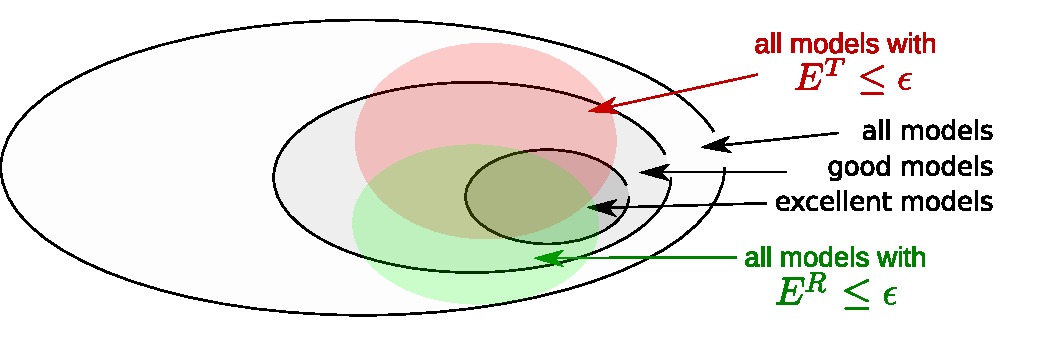
\includegraphics[width=10cm]{img/ModelSelection_models_v2.pdf}
	\end{center}
\end{frame}


% -----------------------------------------------------------------------------
\begin{frame}\frametitle{Regularization example: weight decay}
	\begin{equation*}
		E_{[\vec{w}]}^R \quad=\quad \frac{1}{2} \sum_{(i, j, v', v)} 
			\big( \mathrm{w}_{ij}^{v'v} \big)^2
	\end{equation*}
	%\vspace{2mm}
	
	\begin{center}
		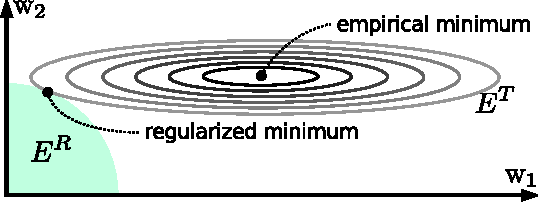
\includegraphics[width=7cm]{img/empirical_vs_regularized}
	\end{center}

	%\vspace{2mm}
	\begin{block}{Minimization of $R$ through gradient descent}
		\begin{equation*}
			\Delta \mathrm{w}_{ij}^{v'v} \quad\sim\quad 
				-\frac{\partial R}{\partial \mathrm{w}_{ij}^{v'v}}
			\quad=\quad - \underbrace{\frac{\partial E^T}%
				{\partial \mathrm{w}_{ij}^{v'v}}}_{
				\substack{\text{e.g. via} \\ \text{backprop}}}
			\;\;-\;\; \underbrace{\lambda \mathrm{w}_{ij}^{v'v}}_{
				\substack{\text{decay} \\ \text{term}}}
		\end{equation*}
	\end{block}
\end{frame}


% -----------------------------------------------------------------------------
\begin{frame}\frametitle{Other forms of regularization}
	\iitem{ general form of regularization: 
		$E^R = \sum\limits_{(i, j, v', v)} {|w_{ij}^{v'v}|}^q$}
	\begin{center}
		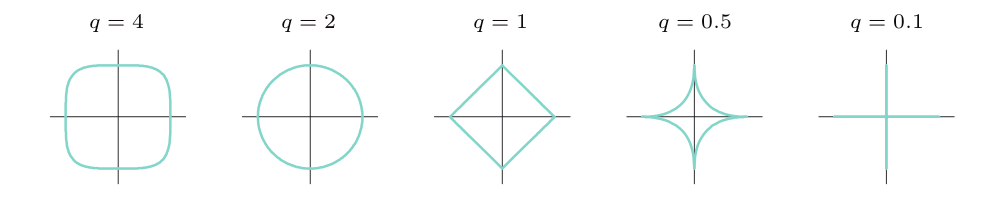
\includegraphics[width=9.5cm]{img/QnormPenalties_clean.png} \\
		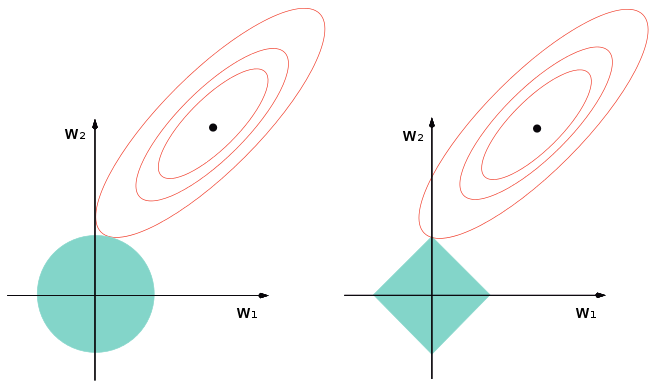
\includegraphics[width=7cm]{img/RegularizationTypesIntersect_clean.png} \\[-2mm]
		{ \footnotesize $L_2$ {\em weight decay} with $q=2$ 
			\hspace{1cm} $L_1$ {\em lasso} with $q=1$ \hspace{1cm} $ $}
	\end{center}

\end{frame}


% -----------------------------------------------------------------------------
\begin{frame}\frametitle{Regularization example: symmetries} 
	Odd vs. even function
	\begin{equation*}
		E_{[\mathrm{w}]}^R = \frac{1}{2p} \sum_{\alpha = 1}^p 
			\Big( y_{(\vec{x}^{(\alpha)}; \vec{w})} 
				\pm y_{(-\vec{x}^{(\alpha)}; \vec{w})} 
			\Big)^2
	\end{equation*}
	\pause
	Invariance under translation:
	\begin{equation*}
		E_{[\mathrm{w}]}^R = \frac{1}{2p} \sum_{\alpha = 1}^p 
			\Big( y_{(\vec{x}^{(\alpha)}; \vec{w})} 
				- y_{(\vec{x}^{(\alpha)} - \vec{t}; \vec{w})} 
			\Big)^2
	\end{equation*}
	\pause
	Monotony:
	\begin{equation*}
		E_{[\mathrm{w}]}^R = \frac{1}{n_p} \sum_{
			\mathrm{x}^{(\alpha)} > \mathrm{x}^{(\beta)}} 
		\left \{
		\begin{array}{cl}
			\Big( y_{(\vec{x}^{(\alpha)}; \vec{w})} - 
				y_{(\vec{x}^{(\beta)}; \vec{w})} \Big)^2  
			& \text{if } y_{(\vec{x}^{(\alpha)}; \vec{w})} < 
				y_{(\vec{x}^{(\beta)}; \vec{w})} \\[2mm] 
			0 & \text{else}
		\end{array} \right.
	\end{equation*}
\end{frame}

% ------------------------------------------------------------------------------
\begin{frame} \frametitle{Early stopping}
	\begin{center}
		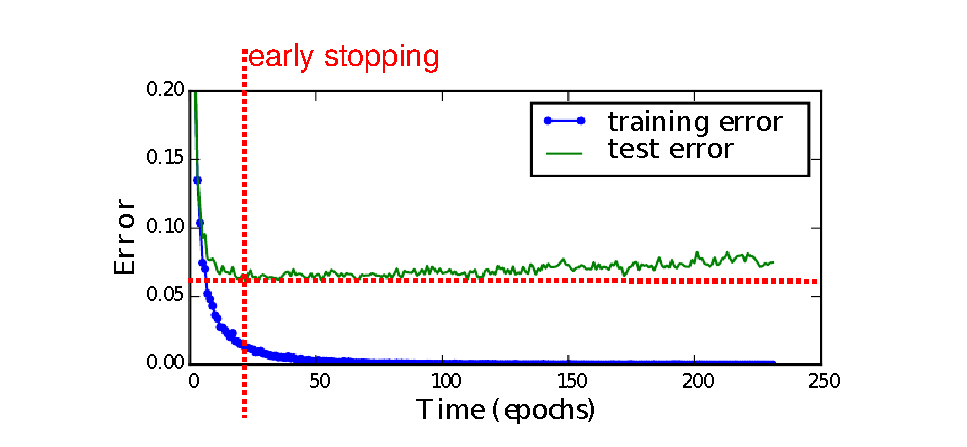
\includegraphics[width=10cm]{img/early_stopping.pdf}
	\end{center}
	\iitem{Estimate generalization error with a test set during training.}
	\iitem{Stop training when the error on the test set rises.}
	\blfootnote{\hfill (trained on MNIST, Goodfellow et al., 2016)}
\end{frame}

% ------------------------------------------------------------------------------


% -----------------------------------------------------------------------------
\begin{frame}\frametitle{Choice of regularization parameter}
	\begin{block}{Testset method}
		\begin{enumerate}
		  \item perform model selection for different values of $\lambda$\\ 
		  		(on training data) 
		  \item<2-> select value of $\lambda$, 
		  		which provides best prediction results\\ 
				(on test data) 
		  \item<3-> estimate generalization performance of selected $\lambda$\\
		  		(on validation data)
		\end{enumerate}
	\end{block}	
	
	\vspace{1cm} 
	
	$ $\hspace{1cm}
	\includegraphics<1->[width=8cm]{img/traintestvalidation.pdf} 
\end{frame}


% -----------------------------------------------------------------------------
\begin{frame}\frametitle{Choice of regularization parameter}
	\begin{block}{$n$-fold cross-validation}
		\For{$\lambda = \lambda_1$ {\em\textbf{to}} $\lambda_n$}{
			perform $n$-fold cross-validation on 
				data with regularization $\lambda$
		}
		\vspace{2mm}

		pick optimal $\lambda^{\text{opt}}$ with minimum $\widehat{E}^G$\\
		\vspace{2mm}

		\textbf{final model:} train network on all data with $\lambda^{\text{opt}}$ 
	\end{block}
	
	\vspace{2mm}
	\begin{center}
		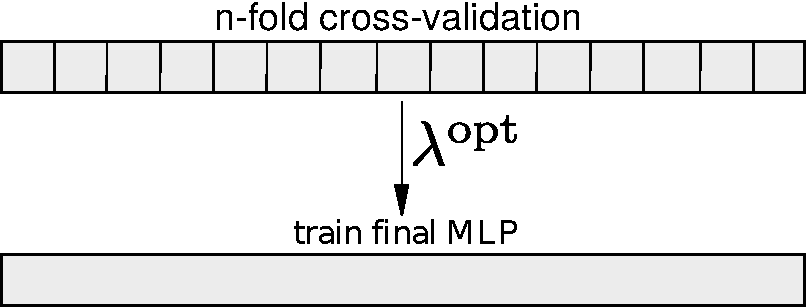
\includegraphics[width=8cm]{img/nfoldcrossvalidation.pdf} 
	\end{center}
\end{frame}


% -----------------------------------------------------------------------------
\begin{frame}\frametitle{Validation}
	\begin{itemize}
	\item[\textcircled{1}]
	$ \begin{array}{ll}
		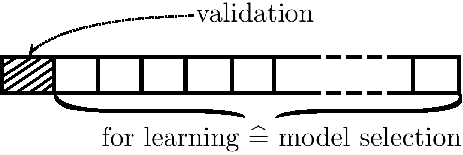
\includegraphics[height=1.2cm]{img/section1_fig34}
		& \begin{array}{ll}
			\bullet & \text{\footnotesize do n - 1 
				cross-validation for all values of } \lambda \\
			\bullet & \text{\footnotesize train with best $\lambda$} \\
			\bullet & \text{\footnotesize validate with learned model}
		\end{array}
	\end{array} $
	%\pause
	\item[\textcircled{2}]
	$ \begin{array}{ll}
		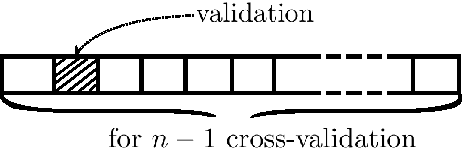
\includegraphics[height=1.2cm]{img/section1_fig35}
		& \begin{array}{ll}
			\bullet & \text{\footnotesize do n - 1 
				cross-validation for all values of } \lambda \\
			\bullet & \text{\footnotesize train with best $\lambda$} \\
			\bullet & \text{\footnotesize validate with learned model}
		\end{array}
	\end{array} $
	%\pause
	\item[\textcircled{n}]
	$ \begin{array}{ll}
		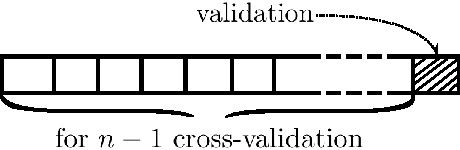
\includegraphics[height=1.2cm]{img/section1_fig36}
		& \begin{array}{ll}
			\bullet & \text{\footnotesize do n - 1
				cross-validation for all values of } \lambda \\
			\bullet & \text{\footnotesize train with best $\lambda$} \\
			\bullet & \text{\footnotesize validate with learned model}
		\end{array}
	\end{array} $
	\end{itemize}
	
	\begin{itemize}
		\item $\widehat{E}^G \quad\corresponds\quad$ 
			average over all $n$ validation errors
	\end{itemize}
\end{frame}


% -----------------------------------------------------------------------------
\begin{frame} 
	\begin{itemize}
		\item Never use test data for model selection 
			(including hyper-parameter search).
		\vspace{4mm}
		\item Always embed the whole selection procedure (including 
			hyper-parameter search) within an $n$-fold cross-validation run.
	\end{itemize}
\end{frame}


\mode*

\clearpage

\mode<all>
\section{Validation}

\begin{frame}\frametitle{\secname}
Recall:
    \mode<article>{
    Fitting an MLP to a desired function $y(\vec x)$ requires the following:
    }

    \begin{enumerate}
    \item 
    \mode<article>{A cost function  with the objective to optimize it, often a minimization problem:}
    \mode<presentation>{A cost function:\vspace{-10mm}}
	\begin{equation}
		e\tyxw \eqexcl \min_{\vec w}
	\end{equation}
    \pause
    \item A performance measure, a criterion for \emph{model selection}.
    \mode<article>{Specifically, \\

    the generalization \textbf{error} $E^G$ which is defined as:}	
    \begin{equation} 
                \EGw \; := \; \left<\,e\,\right>_{y_T, \vec{x}; \vec w} 
                \; = \; \iint d \vec{x} \, dy_T \; 
                    P{(y_T, \vec{x})} \, e{\tyxw}
    \end{equation}
    \pause
    Because $P{(y_T, \vec{x})}$ is not known, \mode<article>{we turn to the principle of empirical risk minimization (ERM).
    According to ERM we can approximate $\EGw$ by computing the} empirical average $\ETw$ using the available training data:
    $$
    \left\{\left(\vec x^{(\alpha)}, y_T^{(\alpha)}\right)\right\}, \alpha=1,\ldots,p
    $$.
    \mode<article>{The training error $\ETw$ becomes:}

    \mode<presentation>{\vspace{-10mm}}
    \begin{equation}
    \text{batch training error:}\quad \ETw=\frac{1}{p}\sum_{\alpha=1}^{p} \underbrace{e\tyxwalpha}_{e^{(\alpha)}}
    \end{equation}
    \mode<article>{
    where $e\tyxwalpha$ (or $e^{(\alpha)}$ for brevity) is the cost computed from the prediction for a specific observation $y(\vec x^{(\alpha)};\vec w)$ and its corresponding label $y_T^{(\alpha)}$. The superscript $^{(\alpha)}$ is used to index a specific point (sample) in the dataset.
    }
    \pause
    \item A model with tunable parameters $\vec w$: MLP, connectionist neuron, \ldots
    \item A learning algorithm\mode<article>{ for finding the set of parameters in our model that will minimize the cost function.\\
    This can be done analytically (depending on some conditions) or through an iterative learning algorithm (e.g. gradient-based learning)}
    \end{enumerate}

\end{frame}

\subsection{Overfitting vs. Underfitting}

\mode*

\clearpage



\mode<all>
\section{Nonlinear basis function}

\subsection{A non-linearly separable problem}

\begin{frame}\frametitle{\subsecname}

\question{Find a linear separation between the classes using only a connectionist neuron.}

\begin{figure}[ht]
     \centering
	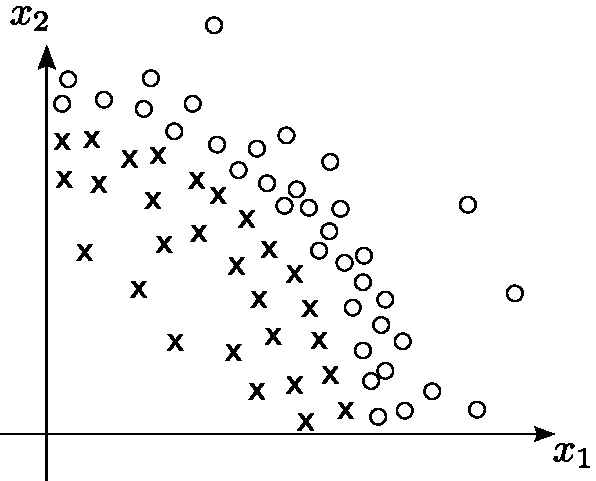
\includegraphics[width=0.4\textwidth]{img/circular}
     \mode<article>{
	\caption{A non-linearly separable classification problem.}
	}
	\label{fig:nonsepcirc} 
\end{figure}

\end{frame}

\begin{frame}\frametitle{\subsecname}

\question{Fit this parabola using only a connectionist neuron.}

\begin{figure}[ht]
     \centering
	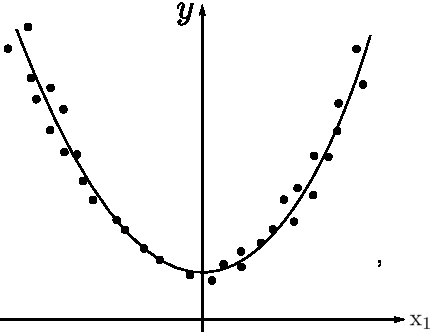
\includegraphics[width=0.4\textwidth]{img/section4_fig11_K2}
     \mode<article>{
	\caption{A non-linearly separable classification problem.}
	}
	\label{fig:nonsepcirc} 
\end{figure}

\question{How would you characterize any parabolic (quadratic) function?}

\pause
\slidesonly{\vspace{-5mm}}
\begin{equation}
y(x) = a x^{2} + b x + c =  w_{2} x^{2} + w_{1} x + w_{0}
\end{equation}

\end{frame}

\subsection{Nonlinear basis function}


\begin{frame}\frametitle{\subsecname}

Feature transformation $(\vec x\in \R^N)$:

\begin{equation}
\vec \phi: \vec x \mapsto \vec \phi(\vec x)
\end{equation}

\mode<article>{$\phi(\vec x)$ can transform our N-dim input $\vec x$ to another feature space of possibly higher dimensionality.
}
Expanding our feature space using \emph{Monomials} of highest degree $k$ (i.e. polynomial expansion):

\begin{align*}
\phi_i(\vec x) \in 
\{\;
&1, 
x_1\,,\, x_2, \ldots, x_N,
x_1^2\,,\, x_1 x_2, \ldots, x_1x_N,\ldots,\,x_N^2,\,\ldots\\
&x_1 x_N^{k-1}\,,\, x_1^k, \ldots, x_N^k
\}
\end{align*}

\begin{equation}
\phi_i(\vec x) \in \Big\{ \prod_{j=1}^N x_j^{a_j} \;\;: a_j \in \N_0 \;\; \text{with} \;\; 0 \, \le \, \sum_{j=1}^{N} a_j \le k  
\Big\} 
\end{equation}

where $i=1,\ldots d$.

Example: $k=9, N=2 \quad \Rightarrow \;\; d=55$


\end{frame}

\subsection{Preprocessing: Sphering}

\begin{frame}\frametitle{\subsecname}

Large $\lVert \vec x \rVert$ can lead to to very large $\phi_i(\vec x)$. \\

We want to decorrelate the transformed data and standardize it (keep variance of $\phi_i(\vec x)$ = 1)
\notesonly{
\emph{Sphering} is a preprocessing step that accomplishes both. 
The sphering transformation yields decorrelated input variables each with unit variance.
}
For every point $\alpha=1,\ldots,p$ from the training set:
\begin{equation}
\vec x^{(\alpha)}_\mathrm{sphered} = \vec \Lambda^{-\frac{1}{2}} \vec E^\top \vec x^{(\alpha)}_\mathrm{centered}.
\end{equation}

Here 
\begin{itemize}
 \item[]   
$\vec x^{(\alpha)}_\mathrm{centered} = \vec x^{(\alpha)} - \big<{\vec x}\big>\quad$ 
\notesonly{
denotes the centered data point $\alpha$ w.r.t. the center of the training data }
$\big<{\vec x}\big> = \frac{1}{p} \sum_{\alpha=1}^p \vec x^{(\alpha)}$,
\item[] $\vec E = (\vec e_1, \dots, \vec e_N)\quad$ is the eigenvector matrix and $\vec \Lambda = \mathrm{diag}(\lambda_1, \dots, \lambda_N)$ is the eigenvalue matrix for the eigendecomposition 
$$
\vec C \, \vec e_i = \lambda_i \vec e_i
$$ of the covariance matrix $\vec C$ with $C_{ij} = \frac{1}{p} \sum_{\alpha=1}^p x^{(\alpha)}_{\mathrm{centered},i} \, x^{(\alpha)}_{\mathrm{centered},j}$.
\end{itemize}


\end{frame}

\begin{frame}\frametitle{\subsecname}

Examining the properties of the data after sphering:

\begin{align}
\frac{1}{p}  \sum_{\alpha=1}^{p} \vec x^{(\alpha)}_\mathrm{sphered} &= \vec 0 \quad \text{(centered)},\\
\frac{1}{p}  \sum_{\alpha=1}^{p} (\vec x^{(\alpha)}_\mathrm{sphered})^{2} &=  1 \quad \text{(unit variance)},\\
\frac{1}{p}  \sum_{\alpha=1}^{p} x^{(\alpha)}_{\mathrm{sphered},i} \, x^{(\alpha)}_{\mathrm{sphered},j} &= 0 \quad \text{(zero covariance)},
\end{align}

\textbf{Important:} Reuse the same pre-processing (centering, sphering) on validation set. \notesonly{Do not recompute a separate mean or sphering transformation for the validation set.}
Also apply to test-set in case of a 3-way split.

\end{frame}

\subsection{Linear neuron for regression: Analytical solution}

\begin{frame}\frametitle{\subsecname}

\underline{Data}:\\

\begin{table}[h]
\begin{tabular}{rl}
transformed input & $\vec \phi^{(\alpha)} := \vec \phi(\vec x^{(\alpha)}) = \big (
\phi_{1}(\vec x^{(\alpha)}), \phi_{2}(\vec x^{(\alpha)}), \ldots, \phi_{d}(\vec x^{(\alpha)}) \big)^{\top}$ \\
label         & $y_{T}^{(\alpha)} \in \R$ \\
with & $\alpha = 1,\ldots,p$ and $\vec x$ has been centered and sphered.
\end{tabular}
\end{table}

\pause

\underline{Model}:\\[-5mm]

\notesonly{linear neuron on the \emph{the transformed} input:}
\begin{equation}
    y(\vec \phi; \vec w) = \vec w^{\top} \vec \phi = \sum_{i=1}^{d} w_{i} \phi_{i}(\vec x)\notesonly{\quad \text{(bias already incl.)}}
\end{equation}

quadratic cost function, L2 regularization. \pause Reuse solution for linear regression:

\begin{equation}
\vec w^{*} = \left( \vec \Phi \, \vec \Phi^{\top} + \lambda \vec I_{d}\right)^{-1} \vec \Phi \, \vec y_{\text{True}}^{\top}
\end{equation}

where $\vec \Phi = \left( \vec \phi^{(1)},\ldots, \vec \phi^{(\alpha)},\ldots, \vec \phi^{(p)}\right) \in \R^{d,p}$

\end{frame}


\mode*

\clearpage

\end{rightcolumn}
\end{paracol}

\end{document}
